\documentclass[12pt,a4paper]{article}

\usepackage[czech]{babel}
\usepackage[utf8]{inputenc}
\usepackage{float}
\usepackage{graphicx}
\usepackage{textcomp}
% rovnice zarovnávat doleva
\usepackage[fleqn]{amsmath}
\usepackage[table,xcdraw]{xcolor}
\usepackage{caption}

% neodsazovat nové odstavce
\setlength{\parindent}{0pt}

\begin{document}

	%%%%%%%%%%%%%%%%%%%%%%%%%%%%%%%%%%%%%%%%%%%%%%%% Titulní list %%%%%%%%%%%%%%%%%%%%%%%%%%%%%%%%%%%%%%%%%%%%%%%%

	\begin{titlepage}
		\begin{center}
			\textsc{\LARGE Vysoké Učení Technické v Brně} \\[0.5cm]
			{\LARGE Fakulta informačních technologií}

			\begin{figure}[H]
				\center\includegraphics[width=0.5\linewidth]{obr/logo.pdf}
			\end{figure}

			\vspace{3cm}

			\textsc{\LARGE Elektronika pro informační technologie} \\[0.5cm]
			\textsc{\LARGE 2016/2017} \\[3.5cm]

			\textbf{{\LARGE Semestrální projekt}}
		\end{center}
		\vfill
		\begin{flushleft} 
			\large
			Dominik Harmim (xharmi00)
			\hfill
			Brno, \today
		\end{flushleft}
	\end{titlepage}

	%%%%%%%%%%%%%%%%%%%%%%%%%%%%%%%%%%%%%%%%%%%%%%%% 1. příklad %%%%%%%%%%%%%%%%%%%%%%%%%%%%%%%%%%%%%%%%%%%%%%%%

	\section*{1.A}

	{\Large Zadání:} \\
	$U_1 = 80 \text{V} \; U_2=120 \text{V}$ \\
	$R_1 = 350 \Omega \; R_2 = 650 \Omega \; R_3 = 410 \Omega \;
	R_4 = 130 \Omega \; R_5 = 360 \Omega \; R_6 =750 \Omega$ \\
	$R_7 = 310 \Omega \; R_8 = 190 \Omega$

	$U_{R_8} = \: \text{?}$ \\
	$I_{R_8} = \: \text{?}$ \\

	\begin{figure}[H] 
		\vspace{-1.1cm}
		\center\includegraphics[width=0.6\linewidth]{obr/1_1}
	\end{figure}

	{\Large Řešení (metoda postupného zjednodušování):}\\

	\begin{figure}[H]
		\vspace{-1.1cm}
		\center\includegraphics[width=1.1\linewidth]{obr/1_2}
		\caption*{transfigurace - trojúhelník \textrightarrow \hspace{0.1cm} hvězda}
	\end{figure}
	\begin{gather*}
		R_A = \frac{R_1  R_2}{R_1 + R_2 + R_3} = \frac{350 \cdot 650}{350 + 650 + 410} = \frac{22750}{141} \Omega \\
		R_B = \frac{R_1  R_3}{R_1 + R_2 + R_3} = \frac{350 \cdot 410}{350 + 650 + 410} \doteq 101.773 \Omega \\ 
		R_C = \frac{R_2  R_3}{R_1 + R_2 + R_3} = \frac{650 \cdot 410}{350 + 650 + 410} = \frac{26650}{141} \Omega
	\end{gather*}

	\begin{figure}[H]
		\center\includegraphics[width=0.6\linewidth]{obr/1_3}
		\caption*{$R_B$ a $R_4$ jsou zapojeny sériově stejně jako $R_C$ a $R_5$}
	\end{figure}
	\begin{gather*}
		R_{B_4} = R_B + R_4 = 101.773 + 130 = 231.773 \Omega \\
		R_{C_5} = R_C + R_5 = \frac{26650}{141} + 360 = \frac{77410}{141} \Omega
	\end{gather*}

	\begin{figure}[H]
		\center\includegraphics[width=0.6\linewidth]{obr/1_4}
		\caption*{$R_{B_4}$ a $R_{C_5}$ jsou zapojeny paralelně}
	\end{figure}
	\begin{gather*}
		R_{B_{4}C_{5}} = \frac{R_{B_4} R_{C_5}}{R_{B_4} + R_{C_5}} = \frac{231.773 \cdot \frac{77410}{141}}{231.773 
		+ \frac{77410}{141}} \doteq 162.9717 \Omega
	\end{gather*}

	\begin{figure}[H]
		\center\includegraphics[width=0.6\linewidth]{obr/1_5}
		\caption*{$R_A$ a $R_{B_{4}C_{5}}$ a $R_6$ jsou zapojeny sériově}
	\end{figure}
	\begin{gather*}
		R_{AB_{4}C_{5}6} = R_A + R_{B_{4}C_{5}} + R_6 = \frac{22750}{141} + 162.9717 + 750 \doteq 1074.3194 \Omega
	\end{gather*}

	\begin{figure}[H]
		\center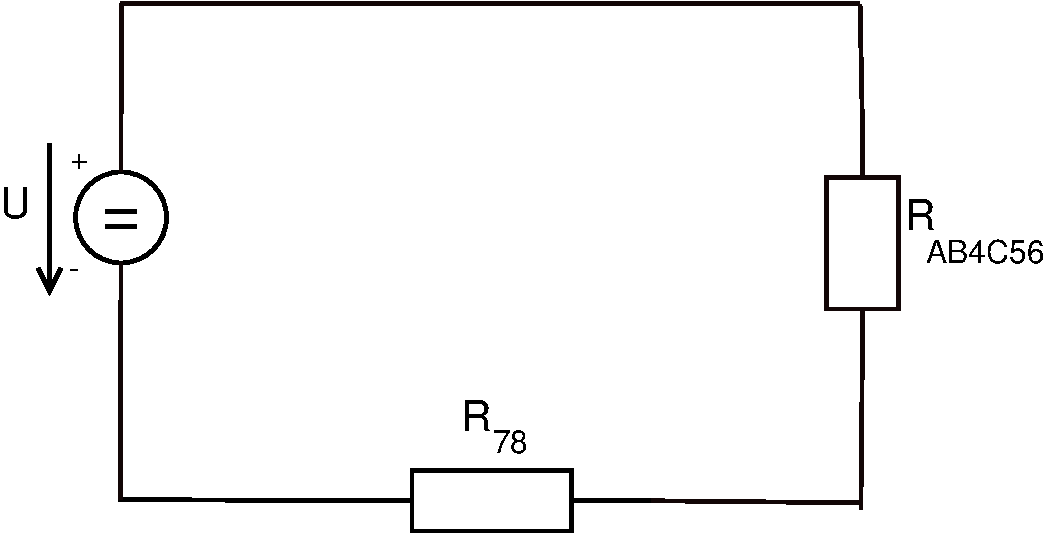
\includegraphics[width=0.6\linewidth]{obr/1_6}
		\caption*{$U_1$ a $U_2$ jsou zapojeny sériově a $R_7$ a $R_8$ jsou zapojeny paralelně}
	\end{figure}
	\begin{gather*}
		U = U_1 + U_2 = 80 + 120 = 200 \text{V} \\
		R_{78} = \frac{R_7 R_8}{R_7 + R_8} = \frac{310 \cdot 190}{310 + 190} = \frac{589}{5} \Omega
	\end{gather*}

	\begin{figure}[H]
		\center\includegraphics[width=0.3\linewidth]{obr/1_7}
		\caption*{$R_{78}$ a $R_{AB_{4}C_{5}6}$ jsou zapojeny sériově -- získáváme $R_{EKV}$}
	\end{figure}
	\begin{gather*}
		R_{EKV} = R_{78} + R_{AB_{4}C_{5}6} = \frac{589}{5} + 1074.3192 = 1192.1194 \Omega
	\end{gather*}

	Celkový proud $I$:
	\begin{gather*}
		I = \frac{U}{R_{EKV}} = \frac{200}{1192.1194} \doteq 167.7684 \text{mA}
	\end{gather*}

	Teď můžeme zpětně dopočítat $U_{R_{78}} \equiv \boldsymbol{U_{R_8}}$ a $\boldsymbol{I_{R_8}}$:
	\begin{gather*}
		\boldsymbol{U_{R_8}} \equiv U_{R_{78}} = I R_{78} = 0.1677684 \cdot \frac{589}{5} = \boldsymbol{19.7631 \textbf{V}} \\
		\boldsymbol{I_{R_8}} = \frac{U_{R_8}}{R_{78}} = \frac{19.7631}{190} \doteq \boldsymbol{104.0163 \textbf{mA}}
	\end{gather*}

	\newpage

	%%%%%%%%%%%%%%%%%%%%%%%%%%%%%%%%%%%%%%%%%%%%%%%% 2. příklad %%%%%%%%%%%%%%%%%%%%%%%%%%%%%%%%%%%%%%%%%%%%%%%%

	\section*{2.G}

	{\Large Zadání:} \\
	$U = 180 \text{V}$ \\
	$R_1 = 315 \Omega \; R_2 = 615 \Omega \; R_3 = 180 \Omega \; R_4 = 460 \Omega \; R_5 = 300 \Omega$

	$U_{R_4} = \: \text{?}$ \\
	$I_{R_4} = \: \text{?}$ \\

	\begin{figure}[H] 
		\vspace{-0.5cm}
		\center\includegraphics[width=0.6\linewidth]{obr/2_1}
	\end{figure}

	{\Large Řešení (Théveninova věta):} \\

	Vypočítáme $\boldsymbol{R_i}$:
	\begin{figure}[H]
		\center\includegraphics[width=0.5\linewidth]{obr/2_2}
		\caption*{bez $R_4$, napěťový zdroj zkratujeme}
	\end{figure}
	\begin{gather*}
		R_i \equiv R_{AB} = \frac{R_3 (\frac{R_1 R_2}{R_1 + R_2} + R_5)}{R_3 + (\frac{R_1 R_2}{R_1 + R_2} + R_5)} =
		\frac{180 \cdot (\frac{315 \cdot 615}{315 + 615} + 300)}{180 + (\frac{315 \cdot 615}{315 + 615} + 300)} \doteq 132.9279 \Omega
	\end{gather*}

	Vypočítáme $\boldsymbol{U_i}$:
	\begin{figure}[H]
		\center\includegraphics[width=0.6\linewidth]{obr/2_3}
		\caption*{bez $R_4$}
	\end{figure}
	Vypočítám $I_B$ metodou smyčkových proudů s přímým sestavením maticové rovnice:
	\begin{gather*}
		\begin{bmatrix}
			R_1 + R_2	&	-R_2 \\
			-R_2		&	R_2 + R_3 + R_5
		\end{bmatrix}
		\cdot
		\begin{bmatrix}
			I_A \\
			I_B
		\end{bmatrix}
		=
		\begin{bmatrix}
			U \\
			0
		\end{bmatrix}
		\\
		\begin{bmatrix}
			930		&	-615 \\
			-615	&	1095
		\end{bmatrix}
		\cdot
		\begin{bmatrix}
			I_A \\
			I_B
		\end{bmatrix}
		=
		\begin{bmatrix}
			180 \\
			0
		\end{bmatrix}
	\end{gather*}
	Vypočítáme determinanty křížovým pravidlem:
	\begin{gather*}
		\Delta = 
		\begin{vmatrix}
			930		&	-615 \\
			-615	&	1095
		\end{vmatrix}
		= 640125 \\
		\Delta_2 = 
		\begin{vmatrix}
			930		&	180 \\
			-615	&	0
		\end{vmatrix}
		= 110700
	\end{gather*}
	Použitím Cramerova pravidla vypočítáme $I_B$:
	\begin{gather*}
		I_B = \frac{\Delta_2}{\Delta} = \frac{110700}{640125} = \frac{492}{2845} \text{A} \\
		U_i \equiv U_{R_3} = I_B R_3 = \frac{492}{2845} \cdot 180 = \frac{17712}{569} \text{V}
	\end{gather*}

	\begin{figure}[H]
		\center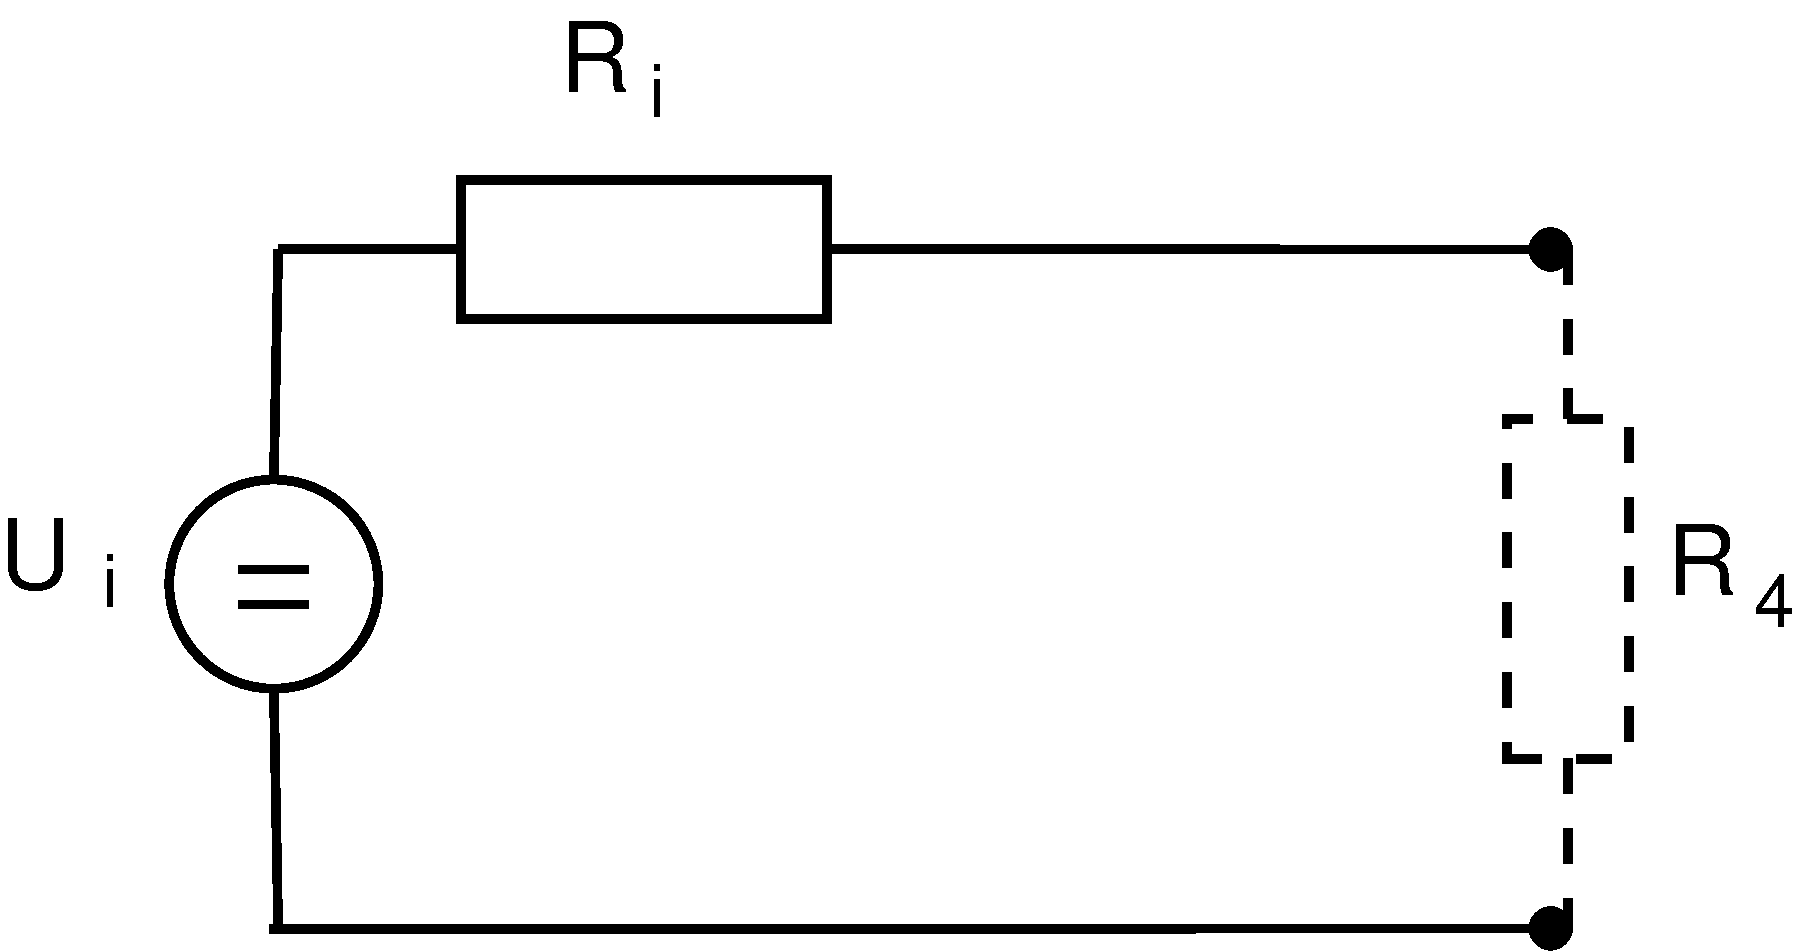
\includegraphics[width=0.6\linewidth]{obr/2_4}
		\caption*{ekvivaletní obvod}
	\end{figure}
	\begin{gather*}
		\boldsymbol{I_{R_4}} = \frac{U_i}{R_i + R_4} = \frac{\frac{17712}{569}}{132.9279 + 460} \doteq \boldsymbol{52.4993 \textbf{mA}} \\
		\boldsymbol{U_{R_4}} = I_{R_4} R_4 = 0.0524993 \cdot 460 \doteq \boldsymbol{24.1497 \textbf{V}}
	\end{gather*}

	\newpage

	%%%%%%%%%%%%%%%%%%%%%%%%%%%%%%%%%%%%%%%%%%%%%%%% 3. příklad %%%%%%%%%%%%%%%%%%%%%%%%%%%%%%%%%%%%%%%%%%%%%%%%

	\section*{3.C}

	{\Large Zadání:} \\
	$U = 110 \text{V}$ \\
	$I_1 = 0.85 \text{A} \; I_2 = 0.75 \text{A}$ \\
	$R_1 = 44 \Omega \; R_2 = 31 \Omega \; R_3 = 56 \Omega \; R_4 = 20 \Omega \; R_5 = 30 \Omega$

	$U_{R_4} = \: \text{?}$ \\
	$I_{R_4} = \: \text{?}$ \\

	\begin{figure}[H] 
		\center\includegraphics[width=0.6\linewidth]{obr/3_1}
	\end{figure}

	{\Large Řešení (metoda uzlových napětí):} \\

	\begin{figure}[H]
		\center\includegraphics[width=0.7\linewidth]{obr/3_2}
		\caption*{přepočítáme napětový zdroj $U$ na proudový zdroj $I_3$ a očíslujeme nezávislé uzly,
		které definují neznámá uzlová napětí}
	\end{figure}
	\begin{gather*}
		G_1 = \frac{1}{R_1} = \frac{1}{44} \text{S} \\
		G_2 = \frac{1}{R_2} = \frac{1}{31} \text{S} \\
		G_3 = \frac{1}{R_3} = \frac{1}{56} \text{S} \\
		G_4 = \frac{1}{R_4} = \frac{1}{20} \text{S} \\
		G_5 = \frac{1}{R_5} = \frac{1}{30} \text{S} \\
		I_3 = \frac{U}{R_5} = \frac{110}{30} = \frac{11}{3} \text{A}
	\end{gather*}

	Sestavíme rovnice pro nezávislé uzly:
	\begin{gather*}
		\text{1)} \; -I_2 + G_1 U_A + G_2 (U_A - U_B) = 0 \\
		\text{2)} \; -I_3 - G_2 (U_A - U_B) + G_3 (U_B - U_C) + G_5 (U_B - U_C) = 0 \\
		\text{3)} \; I_3 - G_3 (U_B - U_C) - G_5 (U_B - U_C) + G_4 U_C + I_1 = 0
	\end{gather*}

	Rovnice upravíme:
	\begin{gather*}
		\text{1)} \; U_A (G_1 + G_2) + U_B (-G_2) = I_2 \\
		\text{2)} \; U_A (-G_2) + U_B (G_2 + G_3 + G_5) + U_C (-G_3 - G_5) = I_3 \\
		\text{3)} \; U_B (-G_3 - G_5) + U_C (G_3 + G_5 + G_4) = -I_3 - I_1
	\end{gather*}

	Přepíšeme rovnice do maticového tvaru:
	\begin{gather*}
		\begin{bmatrix}
			G_1 + G_2	&	-G_2				   &	0 \\
			-G_2 		&	G_2 + G_3 + G_5    &	-G_3 - G_5 \\
			0			&	-G_3 - G_5 		   &	G_3 + G_5 + G_4
		\end{bmatrix}
		\cdot
		\begin{bmatrix}
			U_A \\
			U_B \\
			U_C
		\end{bmatrix}
		=
		\begin{bmatrix}
			I_2 \\
			I_3 \\
			-I_3 - I_1
		\end{bmatrix}
		\\
		\begin{bmatrix}
			\frac{75}{1364}	&	-\frac{1}{31}		  &	0 \\[6pt]
			-\frac{1}{31} 	&	\frac{2173}{26040}    &	-\frac{43}{840} \\[6pt]
			0				&	-\frac{43}{840} 	  &	\frac{17}{168}
		\end{bmatrix}
		\cdot
		\begin{bmatrix}
			U_A \\[6pt]
			U_B \\[6pt]
			U_C
		\end{bmatrix}
		=
		\begin{bmatrix}
			\frac{3}{4} \\[6pt]
			\frac{11}{3} \\[6pt]
			-\frac{271}{60}
		\end{bmatrix}
	\end{gather*}

	Vypočítáme determinanty Sarrusovoým pravidlem:
	\begin{gather*}
		\Delta =
		\begin{vmatrix}
			\frac{75}{1364}	&	-\frac{1}{31}		  &	0 \\[6pt]
			-\frac{1}{31} 	&	\frac{2173}{26040}    &	-\frac{43}{840} \\[6pt]
			0				&	-\frac{43}{840} 	  &	\frac{17}{168}
		\end{vmatrix}
		=
		(\frac{75}{1364} \cdot \frac{2173}{26040} \cdot \frac{17}{168})
		- ((-\frac{43}{840}) \cdot (-\frac{43}{840}) \cdot \frac{75}{1364}) \\
		- (\frac{17}{168} \cdot (-\frac{1}{31}) \cdot (-\frac{1}{31})) = \frac{197}{916608}
		\\
		\Delta_3 =
		\begin{vmatrix}
			\frac{75}{1364}	&	-\frac{1}{31}		  &	\frac{3}{4} \\[6pt]
			-\frac{1}{31} 	&	\frac{2173}{26040}    &	\frac{11}{3} \\[6pt]
			0				&	-\frac{43}{840} 	  &	-\frac{271}{60}
		\end{vmatrix}
		=
		(\frac{75}{1364} \cdot \frac{2173}{26040} \cdot (-\frac{271}{60}))
		+ ((-\frac{1}{31}) \cdot (-\frac{43}{840}) \cdot \frac{3}{4}) \\
		- ((-\frac{43}{840}) \cdot \frac{11}{3} \cdot \frac{75}{1364})
		- ((-\frac{271}{60}) \cdot (-\frac{1}{31}) \cdot (-\frac{1}{31}))
		\doteq -4.4653767 \cdot 10^{-3}
	\end{gather*}

	Použitím Cramerova pravidla vypočítáme $U_C \equiv \boldsymbol{U_{R_4}}$:
	\begin{gather*}
		U_C \equiv \boldsymbol{U_{R_4}} = \frac{\Delta_3}{\Delta} = \frac{-4.4653767 \cdot 10^{-3}}{\frac{197}{916608}}
		\doteq \boldsymbol{-20.7766 \textbf{V}}
	\end{gather*}

	Dopočítáme proud $\boldsymbol{I_{R_4}}$:
	\begin{gather*}
		\boldsymbol{I_{R_4}} = \frac{U_{R_4}}{R_4} = \frac{-20.7766}{20} \doteq \boldsymbol{-1.0389 \textbf{A}}
	\end{gather*}

	\newpage

	%%%%%%%%%%%%%%%%%%%%%%%%%%%%%%%%%%%%%%%%%%%%%%%% 4. příklad %%%%%%%%%%%%%%%%%%%%%%%%%%%%%%%%%%%%%%%%%%%%%%%%

	\section*{4.A}

	{\Large Zadání:} \\
	$u_1 = U_1 \cdot \sin(2 \pi f t) \; u_2 = U_2 \cdot \sin(2 \pi f t)$ \\
	$u_{C_1} = U_{C_1} \cdot \sin(2 \pi f t + \varphi_{C_1})$ \\
	$U_1 = 35 \text{V} \; U_2 = 55 \text{V}$ \\
	$R_1 = 12 \Omega \; R_2 = 14 \Omega \; R_3 = 10 \Omega$ \\
	$L_1 = 120 \text{mH} \; L_2 = 100 \text{mH}$ \\
	$C_1 = 200 \mu \text{F} \; C_2 = 105 \mu \text{F}$ \\
	$f = 70 \text{Hz}$

	$|U_{C_1}| = \: \text{?}$ \\
	$\varphi_{C_1} = \: \text{?}$ \\

	\begin{figure}[H] 
		\vspace{-1.1cm}
		\center\includegraphics[width=0.6\linewidth]{obr/4_1}
	\end{figure}

	{\Large Řešení (metoda smyčkových proudů):} \\

	Vyjádříme si úhlovou frekvenci $\omega$:
	\begin{gather*}
		\omega = 2 \pi f = 2 \pi 70 = 140 \pi \; \text{rad/s}
	\end{gather*}

	Sestavíme maticovou rovnici pro smyčky $I_A$, $I_B$ a $I_C$:
	\begin{gather*}
		\hspace{-2cm}
		\begin{bmatrix}
			R_1 + \omega  L_2 i + R_2 + \omega L_1 i  &  -R_2 - \omega L_1 i  &  -\omega L_2 i \\[6pt]
			-\omega L_1 i - R_2  &  \omega L_1 i + R_2 - \frac{1}{\omega C_2} i - \frac{1}{\omega C_1} i  &  \frac{1}{\omega C_2} i \\[6pt]
			-\omega L_2 i  &  \frac{1}{\omega C_2} i  &  \omega L_2 i + R_3 - \frac{1}{\omega C_2} i
		\end{bmatrix}
		\cdot
		\begin{bmatrix}
			I_A \\[6pt]
			I_B \\[6pt]
			I_C
		\end{bmatrix}
		=
		\begin{bmatrix}
			0 \\[6pt]
			U_1 \\[6pt]
			U_2
		\end{bmatrix}
		\\
		\begin{bmatrix}
			26 + \frac{154}{5} \pi i  &  -14 - \frac{84}{5} \pi i  &  -14 \pi i \\[6pt]
			-14 - \frac{84}{5} \pi i  &  14 + 19.756813 i          &  21.65373 i \\[6pt]
			-14 \pi i                 &  21.65373 i                &  10 + 22.32856 i
		\end{bmatrix}
		\cdot
		\begin{bmatrix}
			I_A \\[6pt]
			I_B \\[6pt]
			I_C
		\end{bmatrix}
		=
		\begin{bmatrix}
			0 \\[6pt]
			35 \\[6pt]
			55
		\end{bmatrix}
	\end{gather*}

	Z této rovnice po řešení Cramerovým pravidlem (s výpočtem determinantů Sarrusovoým pravidlem) vychází:
	\begin{gather*}
		\Delta \doteq 14305.68906 + 10226.73494i \\
		\Delta_2 \doteq -11248.36586 + 57086.89331i \\
		I_B \equiv I_{C_1} = \frac{\Delta_2}{\Delta} = \frac{-11248.36586 + 57086.89331i}{14305.68906 + 10226.73494i}
		\doteq 1.36754 + 3.01289i \text{A}
	\end{gather*}

	Vypočítáme napětí $U_{C_1}$:
	\begin{gather*}
		X_{C_1} = -\frac{1}{\omega C_1} i = -\frac{1}{140 \pi \cdot 200 \cdot 10^{-6}} i \doteq -11.36821i \Omega \\
		U_{C_1} = I_{C_1} X_{C_1} = (1.36754 + 3.01289i) \cdot (-11.36821i) \doteq 34.2511 - 15.5465i \text{V}
	\end{gather*}

	Vypočítáme $\boldsymbol{|U_{C_1}|}$ a $\boldsymbol{\varphi_{C_1}}$:
	\begin{gather*}
		\boldsymbol{|U_{C_1}|} = \sqrt{\operatorname{Re}(U_{C_1})^2 + \operatorname{Im}(U_{C_1})^2} = 
		\sqrt{34.2511^2 + (-15.5465)^2} \doteq \boldsymbol{37.6143 \textbf{V}} \\
		\boldsymbol{\varphi_{C_1}} = \arctan\frac{\operatorname{Im}(U_{C_1})}{\operatorname{Re}(U_{C_1})} =
		\arctan\frac{-15.5465}{34.2511} \doteq \boldsymbol{-0.4261 \textbf{rad}}
	\end{gather*}

	\newpage

	%%%%%%%%%%%%%%%%%%%%%%%%%%%%%%%%%%%%%%%%%%%%%%%% 5. příklad %%%%%%%%%%%%%%%%%%%%%%%%%%%%%%%%%%%%%%%%%%%%%%%%

	\section*{5.G}

	{\Large Zadání:} \\
	$U = 75 \text{V}$ \\
	$L = 50 \text{H}$ \\
	$R = 25 \Omega$ \\
	$i_L(0) = 3 \text{A}$ \\

	$i_L = f(t)$

	\begin{figure}[H] 
		\vspace{-1.2cm}
		\center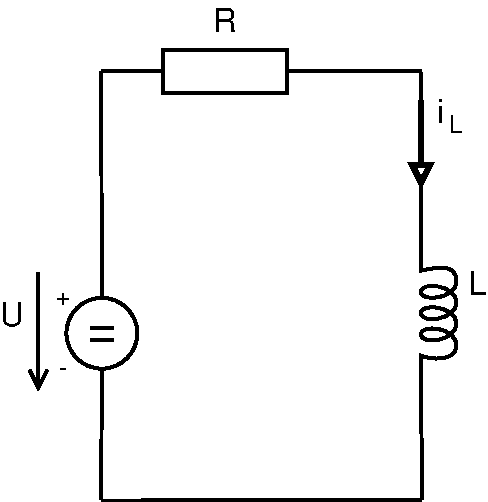
\includegraphics[width=0.4\linewidth]{obr/5_1}
	\end{figure}

	{\Large Řešení (sestavení diferenciální rovnice popisující chování obvodu a výpočet analytického řešení $i_L = f(t)$):} \\

	Sestavíme rovnici pro $i_L'$:
	\begin{gather*}
		i_L' = \frac{U_L}{L}
	\end{gather*}

	Napětí na cívce $U_L$ vyjádříme z rovnice, která platí podle II. Kirchhoffova zákona:
	\begin{gather*}
		U_R + U_L - U = 0 \\
		U_L = U - U_R
	\end{gather*}

	Dosadíme $U_L$ do rovnice pro $i_L'$:
	\begin{gather*}
		i_L' = \frac{U - U_R}{L}
	\end{gather*}

	Po úpravě a dosazení do rovnice dostáváme diferenciální rovnici popisující chování tohoto obvodu:
	\begin{gather*}
		i_L' = \frac{U - R i_L}{L} \\
		L i_L' + R i_L = U \\
		\boldsymbol{50 i_L' + 25 i_L = 75}
	\end{gather*}

	Pro vyřešení diferenciální rovnice vyřešíme charakteristickou rovnici:
	\begin{gather*}
		50 \alpha + 25 = 0 \\
		\alpha = -\frac{25}{50} = -\frac{1}{2}
	\end{gather*}

	Dosadíme $\alpha$ do očekávaného tvaru řešení:
	\begin{gather*}
		i_L(t) = C(t) \cdot e^{\alpha t} \\
		i_L(t) = C(t) \cdot e^{-\frac{1}{2} t} \\
		i_L(t)' = C(t)' \cdot e^{-\frac{1}{2} t} - \frac{1}{2} C(t) \cdot e^{-\frac{1}{2} t}
	\end{gather*}

	Dosadíme $i_L'$ do diferenciální rovnice:
	\begin{gather*}
		50 (C(t)' \cdot e^{-\frac{1}{2} t} - \frac{1}{2} C(t) \cdot e^{-\frac{1}{2} t}) + 25 C(t) \cdot e^{-\frac{1}{2} t} = 75 \\
		50 C(t)' \cdot e^{-\frac{1}{2} t} - 25 C(t) \cdot e^{-\frac{1}{2} t} + 25 C(t) \cdot e^{-\frac{1}{2} t} = 75 \\
		50 C(t)' \cdot e^{-\frac{1}{2} t} = 75 \\
		C(t)' = \frac{3}{2} \cdot e^{\frac{1}{2} t} \\
		C(t) = \int \frac{3}{2} \cdot e^{\frac{1}{2} t} dt = 3 \cdot e^{\frac{1}{2} t} + K
	\end{gather*}

	Dosadíme $C(t)$ do očekávaného tvaru řešení:
	\begin{gather*}
		i_L(t) = (3 \cdot e^{\frac{1}{2} t} + K) \cdot e^{-\frac{1}{2} t} = 3 + K \cdot e^{-\frac{1}{2} t}
	\end{gather*}

	Vypočítáme $K$ podle počáteční podmínky $i_L(0) = 3 \text{A}$:
	\begin{gather*}
		i_L(0) = 3 + K \cdot e^{-\frac{1}{2} \cdot 0} \\
		3 = 3 + K \\
		K = 0
	\end{gather*}

	Dosadíme $K$ do očekávaného tvaru řešení a dostaneme výsledné $i_L$:
	\begin{gather*}
		i_L = 3 + 0 \cdot e^{-\frac{1}{2} t} \\
		\boldsymbol{i_L} = \boldsymbol{3 \textbf{A}}
	\end{gather*}

	{\Large Provedeme kontrolu výsledku} \\
	První podmínka platí, protože řešení odpovídá počáteční podmínce:
	\begin{gather*}
		i_L(0) = 3 \text{A}
	\end{gather*}

	Druhou podmínku ověříme dosazením do sestavené diferenciální rovnice, jejíž výsledek musí vyjít $75 \text{V}$:
	\begin{gather*}
		U = 50 i_L' + 25 i_L \\
		i_L' = (3)' = 0 \\
		U = 50 \cdot 0 + 25 \cdot 3 = 75 \text{V}
	\end{gather*}

	\newpage

	%%%%%%%%%%%%%%%%%%%%%%%%%%%%%%%%%%%%%%%%%%%%%%%% Výsledky %%%%%%%%%%%%%%%%%%%%%%%%%%%%%%%%%%%%%%%%%%%%%%%%

	\section*{Výsledky}

	\begin{table}[H]
		\hspace{-1cm}
		\begin{tabular}{|c|c|c|c|c|}
			\hline \rowcolor[HTML]{CECBCB}
			1	&	2	&	3	&	4	&	5	\\ \rowcolor[HTML]{CECBCB}
			A	&	G	&	C	&	A	&	G	\\ \hline
			$I_{R_8} \doteq 104.0163 \text{mA}$	&	
			$I_{R_4} \doteq 52.4993 \text{mA}$	&	
			$I_{R_4} \doteq -1.0389 \text{A}$	&	
			$|U_{C_1}| \doteq 37.6143 \text{V}$ &	
			$i_L = 3 \text{A}$	\\

			$U_{R_8} \doteq 19.7631 \text{V}$			&	
			$U_{R_4} \doteq 24.1497 \text{V}$			&	
			$U_{R_4} \doteq -20.7766 \text{V}$			&	
			$\varphi_{C_1} \doteq -0.4261 \text{rad}$	&
			-	\\ \hline
		\end{tabular}
	\end{table}
\end{document}
